% =========================
% DIAGNOSTICS (with inline figures)
% =========================
\section{Geometry-based Diagnostics}
\label{sec:diagnostics}

This section operationalizes the signals introduced in \S\ref{sec:method}: (i) \emph{commutators} that surface order-sensitive module pairs and (ii) \emph{inverse-free curvature} that localizes non-commuting transports on the $(\text{position},\text{layer})$ grid. Unless stated, we use the defaults in Table~\ref{tab:exp-setup} (probes $r{=}6$, targets/layer $k{=}8$, neighbors $m{=}6$, thresholds $\tau_\Delta{=}0.10$, $\tau_\kappa{=}0.12$, orbit tolerance $\delta{=}0.02$).

\subsection{Commutators as order-sensitivity diagnostics}
\label{sec:commutators}
\paragraph{Definition and intent.}
For submodules $A,B$ acting on a calibration batch $X$, define
\[
\Delta_{A,B} \;=\; \big\|\,A\!\circ\!B(X)\;-\;B\!\circ\!A(X)\,\big\|_F,
\]
a model-agnostic indicator of \emph{order sensitivity}. Large $\Delta_{A,B}$ suggests reordering/fusing $A,B$ risks output drift, while small $\Delta_{A,B}$ flags candidates for safe fusion or parallel execution.

\paragraph{Computation recipe.}
Choose a module granularity (e.g., attention heads within a layer, or whole sublayers). Evaluate $A(B(X))$ and $B(A(X))$ on the same $X$ (match seeds and dropout state if applicable) and aggregate per pair $(A,B)$ with $\|\cdot\|_F$. Populate a commutator matrix and visualize as a heatmap (Fig.~\ref{fig:comm-heatmap}).

\paragraph{From signal to action.}
Sort pairs by $\Delta_{A,B}$; above a guard $\tau_\Delta$ run sequentially (and log extra verifiers), below $\tau_\Delta$ allow fusion/reorder/parallelization. For intervention trials, define \emph{output drift} $\delta=\|y_{AB}-y_{BA}\|$ under a safe reorder/fuse and report $\rho(\Delta,\delta)$ (trend illustrated in \figref{fig:diagnostic-suite}(b), see \S\ref{sec:metrics}).

% --- FIG: Commutator heatmap (kept) ---
\begin{figure}[th]
\centering
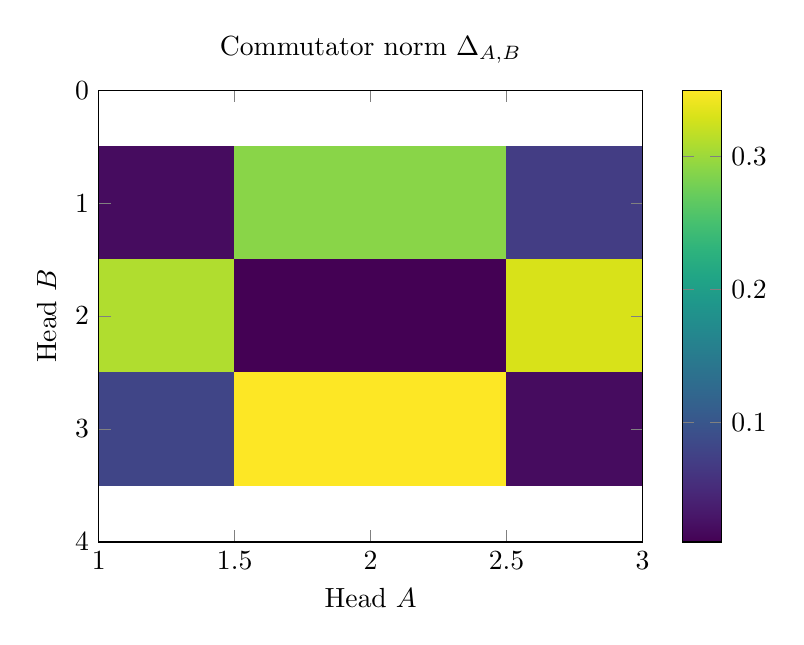
\begin{tikzpicture}
\begin{axis}[
  width=0.7\linewidth,
  view={0}{90},
  colorbar,
  xlabel=Head $A$,
  ylabel=Head $B$,
  title={Commutator norm $\Delta_{A,B}$},
  colormap/viridis,
  enlargelimits=false,
]
\addplot[matrix plot, mesh/rows=3, mesh/cols=3, point meta=explicit] table[meta=z] {
x y z
1 1 0.02
1 2 0.31
1 3 0.08
2 1 0.29
2 2 0.01
2 3 0.35
3 1 0.07
3 2 0.33
3 3 0.02
};
\end{axis}
\end{tikzpicture}
\caption{Heatmap of $\Delta_{A,B}=\|A(B(X))-B(A(X))\|_F$ across attention heads (example data).}
\label{fig:comm-heatmap}
\vspace{-.1in}
\end{figure}

\paragraph{Artifacts.}
Emit \texttt{commutator.csv} with columns \texttt{module\_A, module\_B, delta\_fro}, and a static heatmap for CI. Downstream systems consume $\Delta_{A,B}$ and the guard $\tau_\Delta$.

\subsection{Fiber-bundle perspective: discrete transports and holonomy}
\label{sec:fiber}
\paragraph{Set-up.}
Let the base be $B=\text{Positions}\times\text{Layers}$; each node $(i,\ell)$ carries a fiber $\mathbb{R}^d$. Define \emph{vertical} transports $T^{\text{layer}}_{i,\ell}\approx \partial h_{i,\ell+1}/\partial h_{i,\ell}$ and \emph{horizontal} transports $T^{\text{attn}}_{i\leftarrow j,\ell}\approx \partial h^{\text{out}}_{i,\ell}/\partial h^{\text{in}}_{j,\ell}$ (edge-wise; sparse neighbors). Curvature summarizes the non-commutativity of these transports around small loops; \emph{flat} regions are reordering-safe while \emph{hotspots} are risk zones.

\begin{figure}[t]
\centering
% (figure code unchanged)
\begin{tikzpicture}[>=Latex, x=\DX cm, y=\DY cm]
  % --- grid dots ---
  \foreach \i in {1,...,\Npos} {
    \foreach \l in {0,...,\numexpr\Nlayers-1\relax} {
      \filldraw[black] (\i,\l) circle (\DotSize);
    }
  }
  % --- axis labels (left: layers) ---
  \foreach \l in {0,...,\numexpr\Nlayers-1\relax} {
    \node[anchor=east] at (0.65,\l) {Layer \l};
  }
  % --- axis labels (bottom: positions) ---
  \foreach \i in {1,...,\Npos} {
    \node[anchor=north] at (\i,-0.35) {Pos \i};
  }
  % --- vertical transports (layer edges) ---
  \foreach \i in {1,...,\Npos} {
    \foreach \l in {0,...,\numexpr\Nlayers-2\relax} {
      \draw[->] (\i,\l) -- (\i,\l+1);
    }
  }
  % --- helper macro: horizontal attention arrow ---
  \newcommand{\AttnArrow}[3]{%
    \pgfmathsetmacro{\j}{#1} \pgfmathsetmacro{\ell}{#2} \pgfmathsetmacro{\ii}{#3}
    \path let \p1=(\j,\ell), \p2=(\ii,\ell) in
      coordinate (M) at ($(\p1)!.5!(\p2)$);
    \draw[->,blue!70]
      (\j,\ell) .. controls ($(M)+(0,\AttnLift)$) and ($(M)+(0,\AttnLift)$) .. (\ii,\ell);
  }
  % --- example horizontal transports ---
  \AttnArrow{1}{2}{4}
  \AttnArrow{4}{3}{2}
  \AttnArrow{5}{1}{3}
  % --- holonomy loop rectangle ---
  \draw[red,very thick,rounded corners]
    (\LoopIStart,\LoopLStart) --
    (\LoopIEnd,\LoopLStart) --
    (\LoopIEnd,\LoopLEnd) --
    (\LoopIStart,\LoopLEnd) -- cycle;
  \node[red] at ({(\LoopIStart+\LoopIEnd)/2},{(\LoopLStart+\LoopLEnd)/2}) {$\mathcal{H}$};
\end{tikzpicture}
\caption{Product base \(B=\text{Positions}\times\text{Layers}\). Vertical edges are layer transports \(T^{\mathrm{layer}}_{i,\ell}\); blue curves indicate sample attention transports \(T^{\mathrm{attn}}_{i\leftarrow j,\ell}\). The red rectangle marks a Wilson loop \(\mathcal{H}\) used to measure curvature (order sensitivity).}
\label{fig:fiber-grid}
\vspace{-.1in}
\end{figure}

\paragraph{Curvature maps.}
Aggregate per-loop curvature (below) into position/layer maps (\figref{fig:holonomy-scatter}) and summarize predictiveness by ROC (\figref{fig:diagnostic-suite}(a)); see \S\ref{sec:metrics}.

% --- FIG: Holonomy scatter (kept) ---
\begin{figure}[th]
\centering
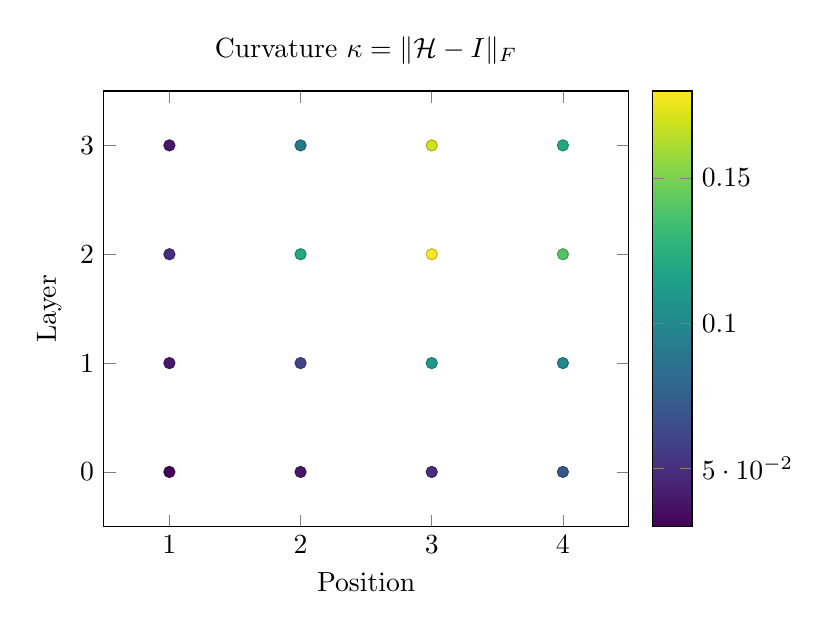
\begin{tikzpicture}
\begin{axis}[
  width=0.68\linewidth,
  colorbar,
  xlabel=Position,
  ylabel=Layer,
  title={Curvature $\kappa=\|\mathcal{H}-I\|_F$},
  colormap/viridis,
  xmin=0.5, xmax=4.5, ymin=-0.5, ymax=3.5,
]
\addplot[
  scatter,
  only marks,
  scatter src=explicit,
  mark=*,
] table[
  row sep=\\,
  x=x, y=y, meta=z,
] {
x y z\\
1 0 0.03\\
2 0 0.04\\
3 0 0.05\\
4 0 0.07\\
1 1 0.04\\
2 1 0.06\\
3 1 0.11\\
4 1 0.10\\
1 2 0.05\\
2 2 0.12\\
3 2 0.18\\
4 2 0.14\\
1 3 0.04\\
2 3 0.09\\
3 3 0.17\\
4 3 0.12\\
};
\end{axis}
\end{tikzpicture}
\caption{Pointwise curvature over (position, layer); color encodes $\kappa$.}
\label{fig:holonomy-scatter}
\vspace{-.1in}
\end{figure}

\subsubsection{Discrete transports: implementation and what curvature measures}
\label{sec:transports-impl}
\paragraph{Vertical maps.}
In pre-LN blocks,
$T^{\text{layer}}_{i,\ell}\!\approx\! I + J^{\text{Attn}}_{i,\ell} + J^{\text{MLP}}_{i,\ell}$,
so residual connections make vertical transport close to identity; curvature therefore captures the \emph{accumulated deviation from identity} around a loop.

\paragraph{Horizontal maps.}
For each candidate edge $(j{\to}i,\ell)$, estimate $T^{\text{attn}}_{i\leftarrow j,\ell}$ by (a) a fast \emph{frozen-softmax} scan using per-head attention weights and $W_V,W_O$, and (b) confirm hotspots with full JVPs. We keep the top-$m$ neighbors by attention mass (with random exploration).

\subsubsection{Inverse-free curvature}
\label{sec:invfree}
\paragraph{Why inverse-free.}
LayerNorm, softmax, and MLPs are not globally invertible, so we avoid $(\cdot)^{-1}$ by comparing two paths that end in the same fiber $(i,\ell{+}1)$:
\[
\kappa_{\mathrm{inv}}(i,j,\ell)^2
= \mathbb{E}_{v}\,\big\|\,T^{\mathrm{layer}}_{i,\ell}T^{\mathrm{attn}}_{i\leftarrow j,\ell}v
- T^{\mathrm{attn}}_{i\leftarrow j,\ell+1}T^{\mathrm{layer}}_{j,\ell}v\,\big\|_2^2,
\]
as defined in Eq.~\eqref{eq:invfree-kappa}. We estimate the expectation with $r$ Rademacher probes via JVPs.

\paragraph{Loop selection and aggregation.}
Sample $k$ target tokens per layer and top-$m$ neighbors to form loops. Aggregate per input with either the maximum $\kappa_{\max}$ or the 95th percentile $\operatorname{p95}(\{\kappa\})$ to obtain a scalar failure predictor; see \S\ref{sec:metrics} and Fig.~\ref{fig:diagnostic-suite}(a).

%\paragraph{Loop selection and aggregation.}
%Sample $k$ target tokens per layer and top-$m$ neighbors to form loops. Aggregate per-input by $\kappa_{\max}$ or percentile (e.g., p95) to obtain a scalar failure predictor; see \S\ref{sec:metrics} and \figref{fig:diagnostic-suite}(a).

\subsubsection{Cost, sparsity, and sampling}
\label{sec:cost-sampling}
\paragraph{Work model.}
With width $d$, layers $L$, tokens $T$, probes $r$, targets/layer $k$, and neighbors $m$,
\[
\text{work}\;\approx\;\mathcal{O}\!\big(r\,L\,k\,m\cdot \mathrm{cost}_{\mathrm{JVP}}\big).
\]
We (i) sample $k$ tokens/layer (uniform or saliency-biased), (ii) keep top-$m$ neighbors, (iii) scan with frozen transports and (iv) confirm hotspots with four JVPs/loop. Defaults: $r{=}6$, $k{=}8$, $m{=}6$.

\subsubsection{Notes and baselines}
\label{sec:notes}
\paragraph{Locality.}
“Locally flat’’ refers to $1{\times}1$ rectangles; $2{\times}2$ loops appear in ablations (rankings typically stable, magnitudes amplified).

\paragraph{Vertical composition.}
Our $T^{\text{layer}}$ already includes residual and sublayers; a two-edge vertical ablation (residual-only then sublayer-only) produces similar hotspot rankings.

\paragraph{Nulls.}
We report curvature for random-initialized models and for shuffled-attention baselines to calibrate magnitudes and false-alarm rates.

\subsection{Gauge fixing for interpretability and CI}
\label{sec:gaugefix}
\paragraph{When and why.}
We apply whitening and Procrustes \emph{for logging and cross-seed comparability}, not when computing $\kappa_{\mathrm{inv}}$. Metrics include probe-accuracy variance across seeds and saliency-rank stability (Kendall-$\tau$). The pipeline (\figref{fig:gauge-pipeline}) standardizes features so CI dashboards are reproducible.

\subsection{Representation tendencies for linguistic transforms}
\label{sec:ling}
\paragraph{Offsets, not theorems.}
Across languages, morphological/syntactic relations often appear as approximately linear offsets in embedding subspaces; this is an empirical tendency, not a claim of an explicit grammar-group representation. We evaluate offset consistency under orthogonal alignment and compare locations of offset-sensitive examples with commutator/curvature hotspots (\figref{fig:diagnostic-suite}(b)).

\medskip
\noindent\textbf{Artifacts and usage.}
This section yields: \texttt{commutator.csv} (pairwise $\Delta_{A,B}$), \texttt{holonomy.csv} (per-loop $\kappa_{\mathrm{inv}}$ with indices $(i,j,\ell)$), and static plots for CI (\figref{fig:comm-heatmap}, \figref{fig:fiber-grid}, \figref{fig:holonomy-scatter},~\figref{fig:diagnostic-suite}(a),~\figref{fig:diagnostic-suite}(b)). Systems consume these along with guard thresholds $(\tau_\Delta,\tau_\kappa)$ to decide when to fuse, reorder, or parallelize, and when to enforce extra verification.
